

\documentclass[10pt,xcolor=dvipsnames]{beamer}\usepackage[]{graphicx}\usepackage[]{color}
%% maxwidth is the original width if it is less than linewidth
%% otherwise use linewidth (to make sure the graphics do not exceed the margin)
\makeatletter
\def\maxwidth{ %
  \ifdim\Gin@nat@width>\linewidth
    \linewidth
  \else
    \Gin@nat@width
  \fi
}
\makeatother

\definecolor{fgcolor}{rgb}{0.345, 0.345, 0.345}
\newcommand{\hlnum}[1]{\textcolor[rgb]{0.686,0.059,0.569}{#1}}%
\newcommand{\hlstr}[1]{\textcolor[rgb]{0.192,0.494,0.8}{#1}}%
\newcommand{\hlcom}[1]{\textcolor[rgb]{0.678,0.584,0.686}{\textit{#1}}}%
\newcommand{\hlopt}[1]{\textcolor[rgb]{0,0,0}{#1}}%
\newcommand{\hlstd}[1]{\textcolor[rgb]{0.345,0.345,0.345}{#1}}%
\newcommand{\hlkwa}[1]{\textcolor[rgb]{0.161,0.373,0.58}{\textbf{#1}}}%
\newcommand{\hlkwb}[1]{\textcolor[rgb]{0.69,0.353,0.396}{#1}}%
\newcommand{\hlkwc}[1]{\textcolor[rgb]{0.333,0.667,0.333}{#1}}%
\newcommand{\hlkwd}[1]{\textcolor[rgb]{0.737,0.353,0.396}{\textbf{#1}}}%
\let\hlipl\hlkwb

\usepackage{framed}
\makeatletter
\newenvironment{kframe}{%
 \def\at@end@of@kframe{}%
 \ifinner\ifhmode%
  \def\at@end@of@kframe{\end{minipage}}%
  \begin{minipage}{\columnwidth}%
 \fi\fi%
 \def\FrameCommand##1{\hskip\@totalleftmargin \hskip-\fboxsep
 \colorbox{shadecolor}{##1}\hskip-\fboxsep
     % There is no \\@totalrightmargin, so:
     \hskip-\linewidth \hskip-\@totalleftmargin \hskip\columnwidth}%
 \MakeFramed {\advance\hsize-\width
   \@totalleftmargin\z@ \linewidth\hsize
   \@setminipage}}%
 {\par\unskip\endMakeFramed%
 \at@end@of@kframe}
\makeatother

\definecolor{shadecolor}{rgb}{.97, .97, .97}
\definecolor{messagecolor}{rgb}{0, 0, 0}
\definecolor{warningcolor}{rgb}{1, 0, 1}
\definecolor{errorcolor}{rgb}{1, 0, 0}
\newenvironment{knitrout}{}{} % an empty environment to be redefined in TeX

\usepackage{alltt}
\setbeamertemplate{navigation symbols}{}



\usepackage{color}
\usepackage{CREAL_slides}
\usepackage[latin1]{inputenc}
\usepackage{calc}
\usepackage[loadonly]{enumitem}
\usepackage{float}





\title[Multivariate methods in health studies]{Methods to integrate multiple tables in biomedical studies to detect biomarkers and stratify individuals \\ \medskip
  \small{Instituto de Salud Carlos III. Centro Nacional de Epidemiolog\'ia \\ September, 2017}}
\author[Juan R Gonzalez]{Juan R Gonzalez}
\institute[CREAL]{BRGE - Bioinformatics Research Group in Epidemiology \\
		  Barcelona Institute for Global Health (ISGlobal) \\
		           {\tt e-mail:juanr.gonzalez@isglobal.org} \\
                  \url{http://www.creal.cat/brge} \\
                  and Departament of Mathematics, UAB
                  }

\date{}
\IfFileExists{upquote.sty}{\usepackage{upquote}}{}
\begin{document}


\frame{\titlepage}


\begin{frame}{Outline}

5-days course aiming to introduce statistical methods and tools to discover new biomarkers and stratify individuals with similar profile from one ore more tables of data 
\begin{itemize}
 \item \textbf{Day 1:} Introduction to R
 \item \textbf{Day 2:} Multivariate methods for one table (non-supervised / supervised)
 \item \textbf{Day 3:} Multivariate methods to integrate multiple tables (I)
 \item \textbf{Day 4:} Multivariate methods to integrate multiple tables (II)
 \item \textbf{Day 5:} DAGs, Mendelian Randomization and mediation analysis to integrate multiple tables
\end{itemize} 
\end{frame}


\begin{frame}\frametitle{Aims of the course}

\begin{figure}
\begin{center}
 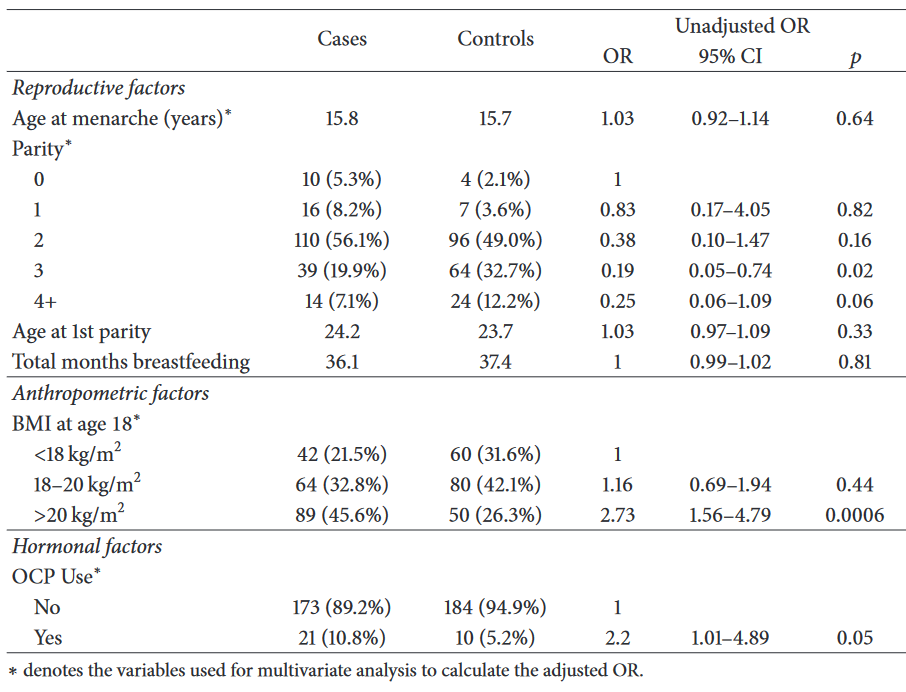
\includegraphics[height=7cm, width=7cm]{figures/step1.png}
\end{center}
\end{figure}

\end{frame}



\begin{frame}\frametitle{Aims of the course}

\begin{figure}
\begin{center}
 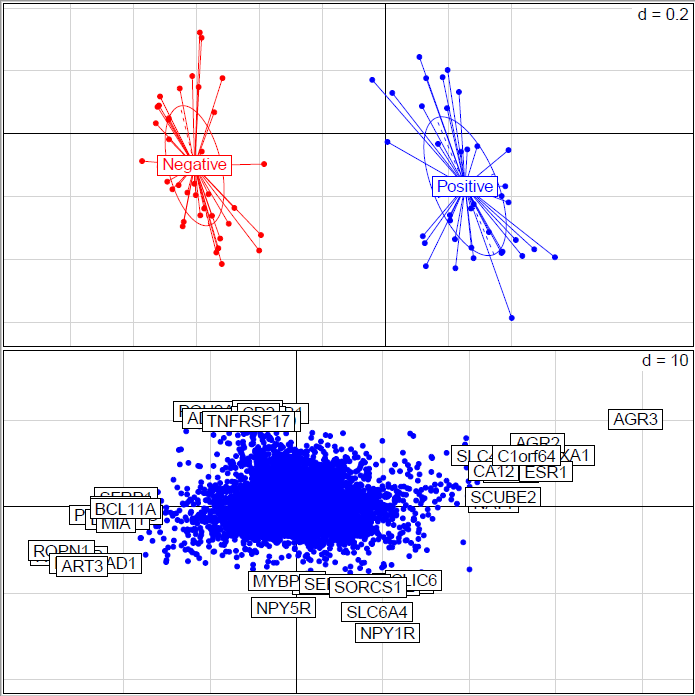
\includegraphics[height=7cm, width=7cm]{figures/step2.png}
\end{center}
\end{figure}

\end{frame}

\begin{frame}\frametitle{Aims of the course}

\begin{figure}
\begin{center}
 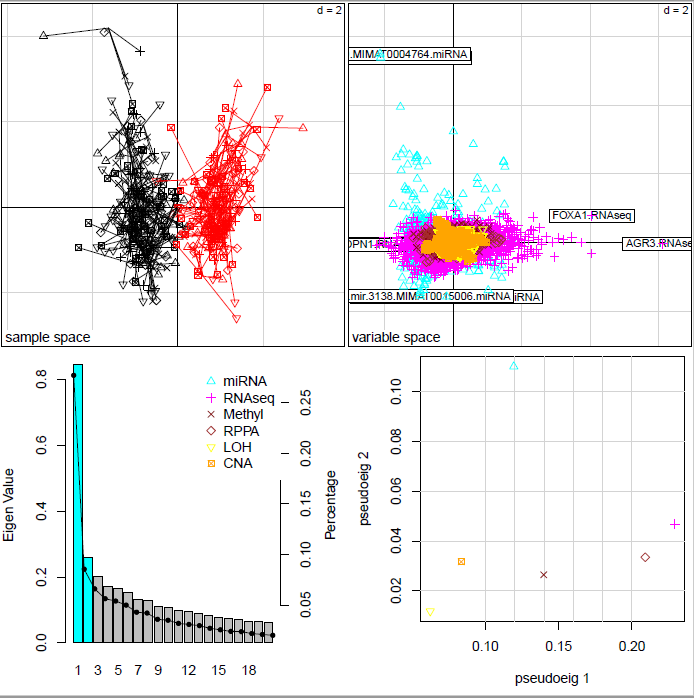
\includegraphics[height=7cm, width=7cm]{figures/step3.png}
\end{center}
\end{figure}

\end{frame}


\begin{frame}\frametitle{Aims of the course}

\begin{figure}
\begin{center}
 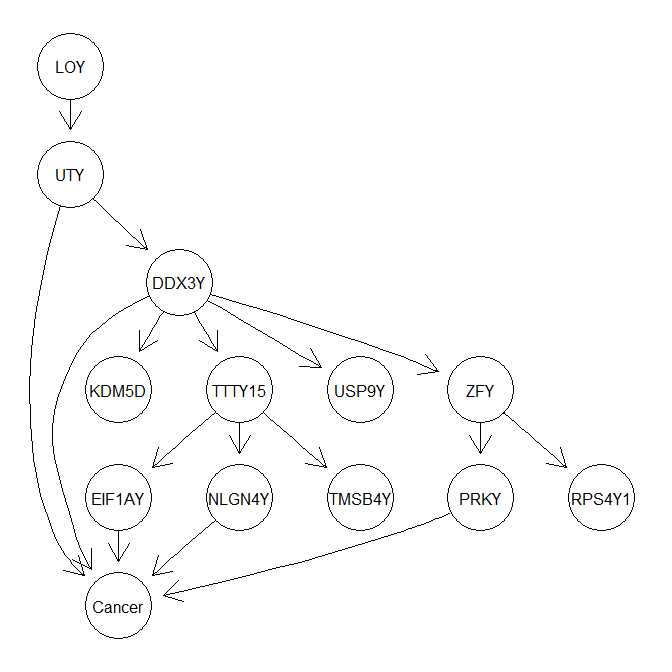
\includegraphics[height=7cm, width=7cm]{figures/step4.png}
\end{center}
\end{figure}

\end{frame}



\begin{frame}\title{Methodology}
 \begin{itemize}
  \item Lectures will introduce statistical methods and how to analyze real data (from different settigs including nutrition, air pollution, genetic, genomics and other biomedical datasets using R packages
  \item Excersises will analyze data from a case/control study in cancer setting were controls and 4 types of cancer (colorectal, stomach, breast and prostate) were studied
  \item Datasets will include a set of variables that are considered as confounding variables, another set about nutrients and a third one ecoding food compsumption variables
  \item Material (including answers to exercises) is available at \url{https://github.com/isglobal-brge/biomarkers_multiple_tables}
 \end{itemize}
 \end{frame}

\end{document}





